\documentclass[kpfonts]{patmorin}
\usepackage{pat}
\usepackage{paralist,graphicx}

\usepackage[utf8]{inputenc}

\usepackage[noabbrev,capitalise]{cleveref}
\crefname{lem}{Lemma}{Lemmas}
\crefname{thm}{Theorem}{Theorems}
\crefname{cor}{Corollary}{Corollaries}
\crefname{prop}{Proposition}{Propositions}
\crefname{conj}{Conjecture}{Conjectures}
\crefname{open}{Open Problem}{Open Problems}
\crefname{obs}{Observation}{Observations}

\crefformat{equation}{(#2#1#3)}
\Crefformat{equation}{Equation #2(#1)#3}

%\theoremstyle{plain}
%\newtheorem{thm}{Theorem}
%\newtheorem{lem}[thm]{Lemma}
%\newtheorem{cor}[thm]{Corollary}
%\newtheorem{prop}[thm]{Proposition}
%\newtheorem{conj}[thm]{Conjecture}
%\newtheorem{open}[thm]{Open Problem}
%\newtheorem{obs}[thm]{Observation}

\usepackage[numbers,sort&compress]{natbib}
\usepackage{hypernat}
\makeatletter
\def\NAT@spacechar{~}
\makeatother

\setlength{\parskip}{1ex}


\newtheorem{property}{Property}
\newcommand{\plabel}[1]{\label{prop:#1}}
\newcommand{\pref}[1]{Property~\ref{prop:#1}}

\DeclareMathOperator{\sn}{sn}
\DeclareMathOperator{\qn}{qn}
\DeclareMathOperator{\sqn}{sqn}
\DeclareMathOperator{\tw}{tw}

\renewcommand{\SS}{\mathcal{S}}

\renewcommand{\le}{\leqslant}
\renewcommand{\leq}{\leqslant}
\renewcommand{\ge}{\geqslant}
\renewcommand{\geq}{\geqslant}

\newcommand{\aref}[1]{(X\ref{a:#1})}
\newcommand{\alabel}[1]{\label{a:#1}}

\title{\MakeUppercase{Stack Number is not Queue-Number Bounded}}

\author{Vida Dujmovi\'c%
	\thanks{School of Computer Science and Electrical Engineering,
		University of Ottawa, Ottawa, Canada (\texttt{vida.dujmovic@uottawa.ca}).
		Research supported by NSERC and the Ontario Ministry of Research and Innovation.}
	,\,\,
	Robert Hickingbotham%
	\thanks{School of Mathematics, Monash University, Melbourne, Australia (\texttt{robert.hickingbotham@monash.edu}).}
	,\,\,
	Pat Morin%
	\thanks{School of Computer Science, Carleton University, Ottawa, Canada (\texttt{morin@scs.carleton.ca}). Research  supported by NSERC and the Ontario Ministry of Research and Innovation.}
	,\,\, 
	David R. Wood\thanks{School of Mathematics, Monash University, Melbourne, Australia (\texttt{david.wood@monash.edu}). Research supported by the Australian Research Council.}
}

\begin{document}
\maketitle

\begin{abstract}
  We describe a family of graphs in which every member has queue number at most 4, but for every integer $s$, there is a member of the family whose stack number is greater than $s$. This resolves open problems of ??? and Blankenship and Oporwoski (???).
\end{abstract}

\section{Introduction}

STACKS vs QUEUES

LINEAR LAYOUTS, CROSSINGS AND NESTINGS

STACKS AND QUEUES

STACK-NUMBER AND QUEUE-NUMBER

BOUNDED PARAMETERS

IMPORTANT PAPERS \citep{HLR92,CLR87,Pupyrev20,DujWoo05,HR92}

IS STACK-NUMBER BOUNDED BY QUEUE-NUMBER? 

\citet{HLR92} showed that every 1-queue graph has a 2-stack layout. 
\citet{HLR92} showed that the ternary hypercubes requires exponentially more stacks than queues. In particular, $n$-vertex ternary hypercubes have queue-number at most $2 \log_3 n$, but stack-number at least $\Omega(n^{1/9-\epsilon})$ for any $\epsilon>0$. We prove the following theorem, which shows that stack-number is not bounded by queue-number. 

\begin{thm}\label{family}
%  There exists a family $\mathcal{F}$ of graphs for which $\qn(G)\le 4$ for every $G\in\mathcal{F}$, and for every $s\in\N$, there exists $G\in\mathcal{F}$ for which $\sn(G)>s$.
 For every $s\in \N$ there exists a graph $G$ with $\qn(G)\le 4$ and $\sn(G)>s$.  
\end{thm}

IS QUEUE-NUMBER BOUNDED BY STACK-NUMBER?

\citet{HLR92} showed that every 1-stack graph has a 2-queue layout. \citet{DJMMUW20} showed that planar graphs have bounded queue-number. In particular, 2-stack graphs have bounded queue-number. It is open whether 3-stack graphs have bounded queue-number. In fact, the case of three stacks is as hard as the general question. \citet{DujWoo05} proved that queue-number is bounded by stack-number if and only if 3-stack graphs have bounded queue-number. Moreover, if this is true then stack-number is bounded by a polynomial function of queue-number.

BLANKENSHIP AND OPOROWSKI CONJECTURE \citep{BO99,BO01}


%Specifically,
%\[
%    \mathcal{F} := \{ S_B\square Q_n : B,Q\in\N\}
%\]
%where $S_B$ denotes the star with $B$ leaves and $Q_n$ is the triangulated $n\times n$ grid.

The graph $G$ in \cref{family} is obtained as follow. Let $S_B$ denote the star graph with root $r$ and $B$ leaves.  Let $Q_n$ be the $n\times n$ triangulated grid, defined by $V(Q):=\{1,\ldots,n\}^2$ and
\begin{align*}
E(Q) & :=\{(x,y)(x+1,y):x\in\{1,\ldots,n-1\},\,y\in\{1,\ldots,n\}\} \\
& \qquad \cup \{(x,y)(x,y+1):x\in\{1,\ldots,n\},\,y\in\{1,\ldots,n-1\}\} \\
& \qquad \cup \{(x,y)(x+1,y+1):x,y\in\{1,\ldots,n-1\}\} \enspace .
\end{align*}
We consider the graph $G:=S_B\square Q_n$. That is, $V(G)=V(S_B)\times V(Q_n)$ where vertices $(v_1,w_1),(v_2,w_2)\in V(G)$ are adjacent whenever $v_1=w_1$ and $v_2w_2\in E(Q_n)$, or $v_1w_1\in E(S_B)$ and $v_2=w_2$. 

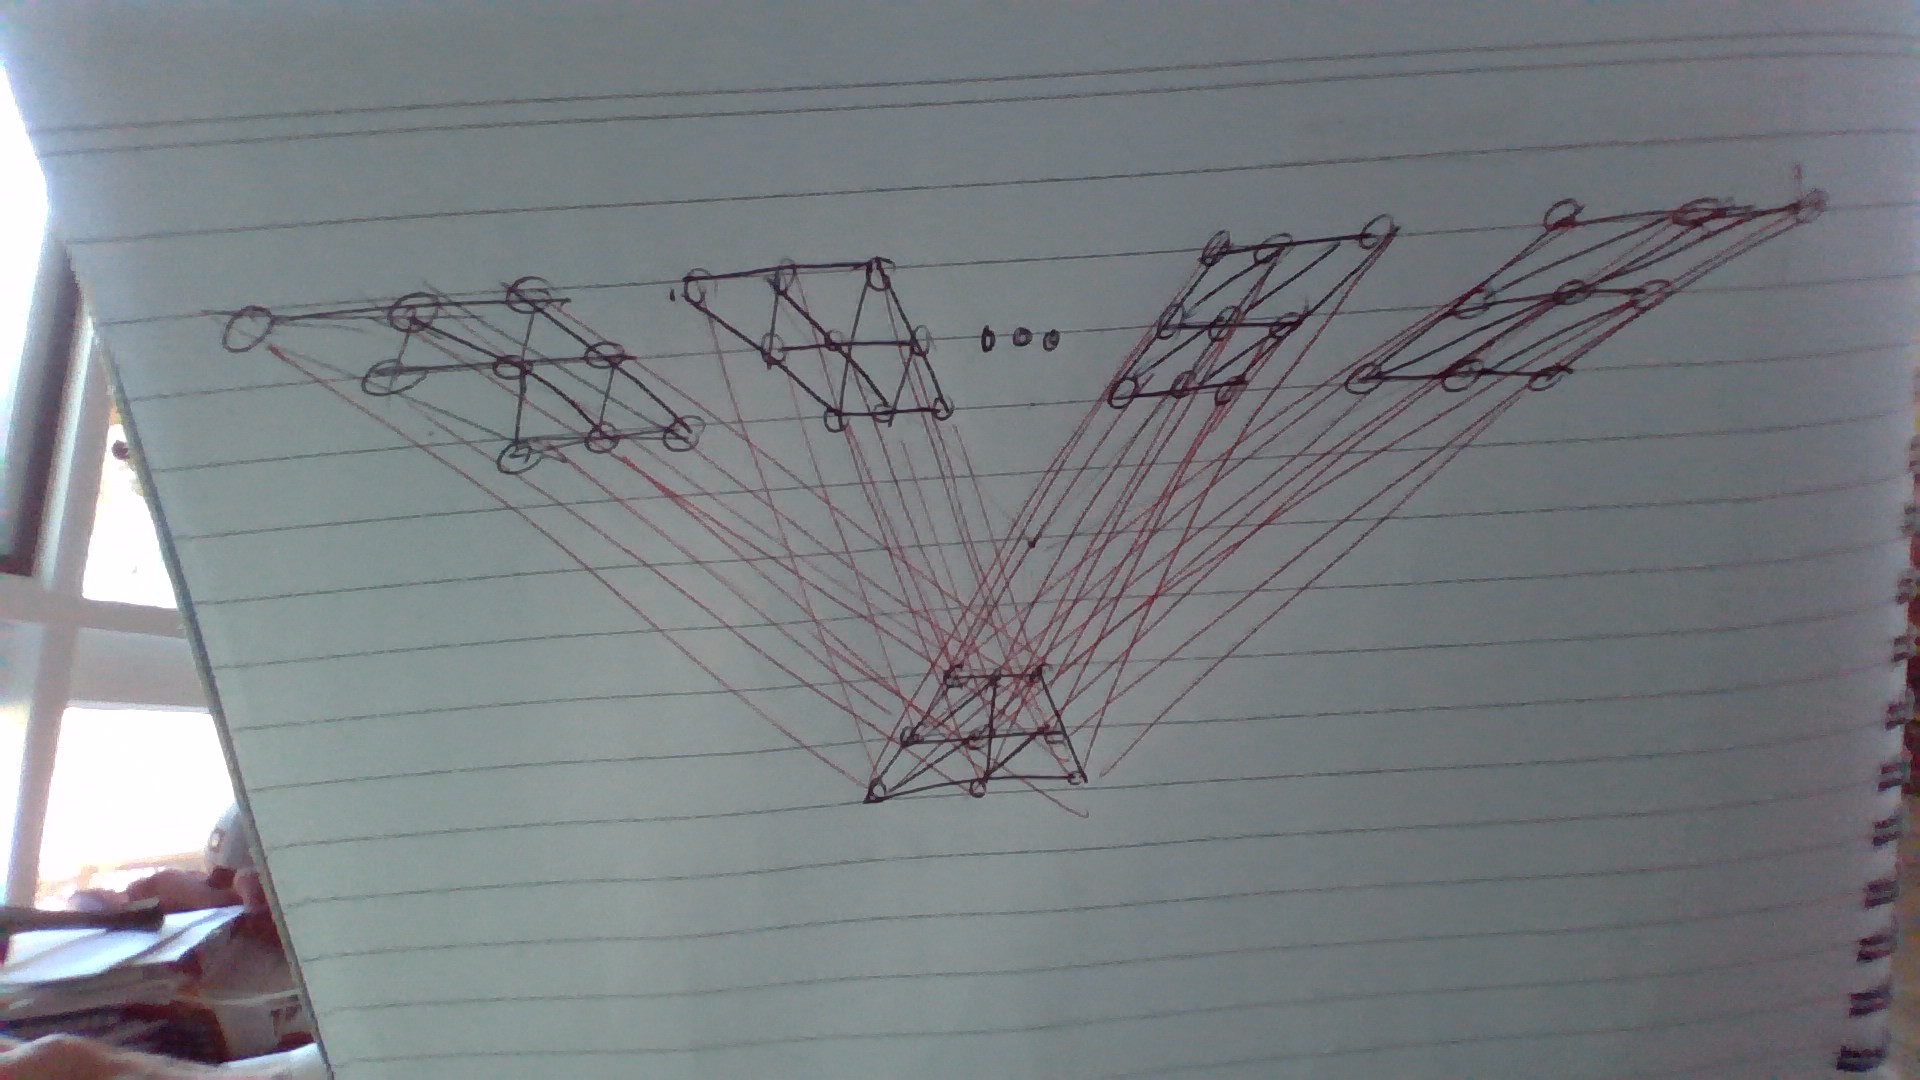
\includegraphics[width=\textwidth]{figs/figure}


\section{Queue-Number Upper Bound}

To prove that $\qn(G)\leq 4$ in Theorem~\ref{family} we need the following definition due to \citet{Wood-Queue-DMTCS05}. A queue layout $(\varphi,\prec)$ is \emph{strict} if for every vertex $u\in V(G)$ and for all neighbours $v,w\in N_G(u)$ with $u\prec v,w$ or $v,w \prec u$, we have $\phi(uv)\neq \phi(uw)$. Let $\sqn(G)$ be the minimum integer $k$ such that $G$ has a strict $k$-queue layout. 
Note that $\sqn(Q_n) \leq 3$: Order the vertices row-by-row and then left-to-right within a row, with vertical edges in one queue, horizontal edges in one queue, and diagonal edges in another queue. 
\citet{Wood-Queue-DMTCS05} proved that $\qn(G \square H) \leq \qn(G) + \sqn(H)$ for all graphs $G$ and $H$. Of course, $S_B$ has a 1-queue layout (since no two edges are nested for any vertex-ordering). Thus 
$$\qn(S_B \square Q_n)\leq 4.$$


ADD TO DISCUSSION LATER:	$Q$ is planar with a Hamiltonian cycle (assuming $n$ is even), so $\sn(Q) \leq 2$


\section{Stack-Number Lower Bound}

Consider a hypothetical $s$-stack layout $(\varphi,\prec)$ of $G$ where $n$ and $B$ are chosen sufficiently large compared to $s$ as detailed below. 

For each node $v$ of $S_b$, we define $\pi_v$ as the permutation of $\{1,\ldots,n\}^2$ in which $(x_1,y_1)$ appears before $(x_2,y_2)$ if and only $(v,x_1,y_1)\prec (v,x_2,y_2)$.  The following lemma is an immediate consequence of the Pigeonhole Principle:

\begin{lem}\lemlabel{uniform_order}
    There exists a permutation $\pi$ of $\{1,\ldots,n\}^2$ and a set $L_1$ of leaves of $S_B$ of size $B_1\ge \lceil B/(n^2)!\rceil$ such that $\pi_{v}=\pi$ for each $v\in L_1$.
\end{lem}

For each leaf $v$ in $L$, consider the subgraph $Q_v$ of $G$ induced by the vertex set $\{(v,x,y):x,y\in\{1,\ldots,n\}$.  The edge colouring $\varphi$ used in the stack layout gives an edge colouring of $Q_v$ using $s$ colours.  The graph $Q_v$ is isomorphic to $Q$, so the edge colouring of $Q_v$ defines an edge colouring of $Q$.  We call this colouring of $Q$ $\varphi_v:Q\to\{1,\ldots,s\}$.  The graph $Q$ has less than $7n^2$ edges, so there are fewer than $s^{7n^2}$ edge colourings of $Q$.  Another application of the Pigeonhole Principle proves the following:

\begin{lem}\lemlabel{uniform_colour}
    There exists a subset $L_2\subseteq L_1$ of size $B_2\ge B_1/s^{7n^2}$
    and an edge colouring $\varphi_0:Q\to\{1,\ldots,s\}$ such that $\varphi_v=\varphi_0$ for each $v\in L_2$.
\end{lem}



\begin{lem}\lemlabel{forward_or_backward}
    There exists a sequence $L_3:=u_1,\ldots,u_{B_3}$ with $\{u_1,\ldots,u_{B_3}\}\subseteq L_2$ of length $B_3\ge (B_2)^{1/2^{n^2-1}}$ such that, for each $p\in V(Q)$, $(u_1,p)\prec (u_2,p)\prec\cdots\prec (u_{B_3},p)$ or $(u_1,p)\succ (u_2,p)\succ\cdots\succ (u_{B_3},p)$.
\end{lem}

\begin{proof}
    Let $p_1,\ldots,p_{n^2}$ denote the vertices of $Q$, in any order.
    Begin with the sequence $S_1:=v_{1,1},\ldots,v_{1,b}$ that contains all $b_1:=B_2$ elements of $L_2$ ordered so that $(v_{1,1},p_1)\prec\cdots(v_{1,b},p_1)$.  For each $i\in\{2,\ldots,n^2\}$, the Erd\H{o}s-Szekeres Theorem implies that, $S_{i-1}$ contains a subsequence $S_i:=v_{i,1},\ldots,v_{i,b_i}$ of length $b_i\ge \sqrt{|S_{i-1}|}$ such that $(v_{i,1},p_i)\prec\cdots\prec(v_{i,b_i},p_i)$ or $(v_{i,1},p_i)\succ\cdots\succ(v_{i,b_i},p_i)$.  It is straightforward to verify by induction that $b_i \ge B_3^{1/2^{i-1}}$ resulting in a final sequence $S_{n^2}$ of length at least $B_2^{1/2^{n^2-1}}$.
\end{proof}

Let $d=B_3$ and let $S_d$ be the the subgraph of $S_b$ induced by $\{r\}\cup\{u_1,\ldots,u_{d}\}$ where $u_1,\ldots,u_d$ is the sequence of leaves defined in \lemref{forward_or_backward}.  Consider the vertex colouring of $Q$ obtained by colouring each vertex $p\in V(Q)$ \emph{red} if $(u_1,p)\prec\cdots\prec (u_d,p)$ and colouring $p$ \emph{blue} if $(u_1,p)\succ\cdots\succ(u_d,p)$.

\begin{lem}\lemlabel{hex_lemma}
    The graph $Q$ contains an $n$-vertex path $R$ consisting entirely of red vertices or entirely of blue vertices.
\end{lem}

\begin{proof}
    The dual of $Q$ is the board on which the game Hex is played.  The well-known \emph{Hex Lemma} states that any colouring of the vertices of $Q$ with colours red and blue contains exactly one of the following \cite{Gale79}:
    \begin{compactenum}
        \item a path with endpoints $(x,1)$ and $(x',n)$ consisting entirely of red vertices, for some $x,x'\in\{1,\ldots,n\}$; or
        \item a path with endpoints $(1,y)$ and $(n,y')$ consisting entirely of blue vertices, for some $y,y'\in\{1,\ldots,n\}$.
    \end{compactenum}
    In either case, the path contains at least $n$ vertices and therefore has a $n$-vertex subpath consisting entirely of red vertices or entirely of blue vertices.
\end{proof}

Without loss of generality, assume that the path $R:=p_1,\ldots,p_n$ defined by \lemref{hex_lemma} consists entirely of red vertices, so that $(u_1,p_j)\prec\cdots\prec (u_d,p_j)$ for each $j\in\{1,\ldots,n\}$.
Recall that $(\varphi,\prec)$ is a hypothetical $s$-stack layout of $G$ and therefore it is also an $s$-stack layout of the subgraph $X:=S_d\square R$.  The following result finishes the proof by showing that this is not possible when $n> 2s$ and $d> s2^{2s+1}$.

\begin{lem}
    The graph $X$ contains a set of edges of size at least $\min\{d/2^{n},n\}/2$ that are pairwise crossing with respect to $\prec$.
\end{lem}

\begin{proof}
    We will define two sequences of nested sets $A_1\supseteq A_1\supseteq A_{n}$ of leaves of $S_d$ so that each $A_i$ satisifies the following conditions:
    \begin{compactenum}[(C1)]
        \item $A_i$ contain $d_i\ge d/2^i$ leaves of $S_d$.
        \item Each leaf $v\in A_i$ defines an $i$-element vertex set $Z_{i,v}:=\{(v,p_j):j\in\{1,\ldots,i\}\}$.  For any distinct $v,w\in A_i$, $Z_{i,v}$ and $Z_{i,w}$ are separated with respect to $\prec$.  In other words, $Z_{i,v}\prec Z_{i,w}$ or $Z_{i,v}\succ z_{i,w}$.
    \end{compactenum}

    Before defining $A_1,\ldots,A_n$ we first show how the existence of the set $A_n$ implies the lemma.  To avoid triple-subscripts, let $d':=d_n\ge d/2^n$.   The set $A_n$ defines vertex sets $Z_{n,v_1}\prec\cdots\prec Z_{n,v_{d'}}$.  Recall that $r$ is the root of $S_b$ so it is adjacent to each of $v_{1},\ldots,v_{d'}$ in $S_b$.  Therefore, for each $j\in\{1,\ldots,n\}$ and each $i\in\{1,\ldots,d'\}$, the edge $(r,p_j)(v_i,p_j)$ is in $X$. Therefore, $(r,p_j)$ is adjacent to an element of each of $Z_{n,v_1},\ldots,Z_{n,v_{d'}}$.

    Since $Z_{n,v_1},\ldots,Z_{n,v_{d'}}$ are separated with respect to $\prec$, when viewed from afar, this situation looks like a complete bipartite graph $K_{n,d'}$ with the root vertices $L:=\{(r,p_j):j\in\{1,\ldots,n\}\}$ in left part and the groups $R:=Z_{n,v_1}\cup\cdots\cup Z_{n,v_{d'}}$ in the right part.  Any linear ordering of $K_{n,d'}$ has a large set of pairwise crossing edges so, intuitively, the graph induced by $L\cup R$ should also have a large set of pairwise crossing edges. \lemref{twister}, below, formalizes this and shows that this graph has a set of at least $\min\{d',n\}/2$ pairwise crossing edges.

    All that remains is to define the sets $A_1\supseteq\cdots\supseteq A_n$.  The set $A_1$ contains all the leaves of $S_d$.  For each $i\in\{2,\ldots,n\}$, the set $A_i$ is defined as follows:  Let $Z_1,\ldots,Z_r$ denote the sets $\{\{(v,p_j):j\in\{1,\ldots,i-1\}\}:v\in A_{i-1}$ ordered so that $Z_1\prec\cdots\prec Z_r$. Label the vertices of $A_{i-1}$ $v_1,\ldots,v_r$ so that $(v_1,p_{i-1})\prec\cdots\prec (v_r,p_{i-1})$. (This is equivalent to naming them so that $(v_j,p_j)\in Z_j$ for each $j\in\{1,\ldots,r\}$.)

    Now we define the set $A_i:=\{v_{2k+1}:k\in\{0,\ldots,\lfloor(r-1)/2\rfloor\}$.  All that remains is to verify that $A_i$ satisfies (C1) and (C2).  To see that $A_i$ satisfies (c1) just observe that $|A_i|=\lceil r/2\rceil \ge r/2= |A_{i-1}|/2\ge d/2^{i}$.  All that remains is to show that $A_i$ satisfies (C2).

    For each $j\in\{i-1,i\}$, let $Q_j:=\{(v,p_j):v\in A_{i-1}\}$.
    Recall that, for each $v\in A_{i-1}$, the edge $e_v:=(v,p_{i-1})(v,p_i)$ is in $X$.  We have the following properties:
    \begin{compactenum}[(P1)]
        \item By \lemref{uniform_colour}, $\varphi(e_v)=\varphi_0(p_{i-1},p_i)$ does not depend on $v$.  In particular for distinct $v,w\in A_{i-1}$ the edges $e_v$ and $e_w$ do not cross.
        \item By the application of \lemref{hex_lemma} the order of vertices in $Q_{i-1}$ by $\prec$ is identical to the order of vertices in $Q_i$ by $\prec$.  That is $(v,p_{i-1})\prec (w,p_{i-1})$ if and only if $(v,p_{i})\prec (w,p_{i})$ for each $v,w\in A_{i-1}$.
        \item By \lemref{uniform_order}, $(v,p_{i-1})\prec (v,p_i)$ for every $v\in A_{i-1}$ or $(v,p_{i-1})\succ (v,p_i)$ for every $v\in A_{i-1}$.
    \end{compactenum}
    These three conditions imply that the vertex sets $Q_{i-1}$ and $Q_{i}$ interleave perfectly with respect to $\prec$. More precisely,
    \[
        (v_1,p_{i-1+b})\prec (v_1,p_{i-b}) \prec (v_2,p_{i-1+b}) \prec (v_2,p_{i-b}) \cdots \prec (v_r,p_{i-1+b}) \prec (v_r,p_{i-b})
    \]
    for some $b\in\{0,1\}$.  Suppose, without loss of generality that $b=0$. [TODO: Explain why (P1)--(P3) imply a perfect interleave.]

    For each odd $j\in\{1,\ldots,r-2\}$ we have $(v_j,p_i)\prec (v_{j+1},p_{i-1}) \prec Z_{j+2}$.  Therefore $Z_j\cup\{(v_j,p_i)\} \prec Z_{j+2}$.  By a symmetric argument, $Z_j\cup\{(v_j,p_i)\} \succ Z_{j-2}$ for each odd $j\in\{3,\ldots,r\}$.  Finally, since $(v_{j},p_i)\prec (v_{j+2},p_i)$ for each odd $i\in\{1,\ldots,r\}$, we have $Z_{j}\cup\{(v_j,p_i)\} \prec Z_{j+2}\cup\{(v_{j+2},p_i)\}$ for each odd $j\in\{1,\ldots,r-2\}$.  Thus $A_i$ satisifies (C2) since the sets $Z_1\cup\{(v_1,p_i)\},Z_3\cup\{(v_3,p_i)\},\ldots,Z_{2\floor (r-1)/2\rfloor+1} \cup (v_{2\floor (r-1)/2\rfloor+1},p_i)$ are precisely the sets $Z_{i,1},\ldots,Z_{i,d_i}$ determined by our choice of $A_i$.
\end{proof}

\begin{lem}\lemlabel{twister}
    Let $G$ be any graph, let $\prec$ be any linear ordering of $V(G)$,  let $Z_{1}\prec\cdots\prec Z_{2s}$ be subsets of $V(G)$, and let $r_1\prec\cdots\prec r_{2s}$ be vertices of $G$ such that, for each $i,j\in\{1,\ldots,2s\}$, $G$ contains an edge $r_iz_j$ with $z_j\in Z_j$. Then $G$ contains a set of $s$ edges that are pairwise crossing with respect to $\prec$.
\end{lem}

\begin{proof}
    At least one of the following two cases applies:
    \begin{enumerate}
        \item $Z_s\prec r_{s+1}$ in which case the graph between $r_{s+1},\ldots,r_{2s}$ and $Z_1,\ldots,Z_s$ has a set of $s$ pairwise-crossing edges.
        \item $r_{s}\prec Z_{s+1}$ in which case the graph between $r_1,\ldots,r_s$ and $Z_{s+1},\ldots,Z_{2s}$ has a set of $s$ pairwise-crossing edges. \qedhere
    \end{enumerate}
\end{proof}

\section{Open Problems}

Recall that every 1-queue graph has a 2-stack layout \citep{HLR92} and we proved that there are 4-queue graphs with unbounded stack-number. The following questions remain open: Do 2-queue graphs have bounded stack-number? Do 3-queue graphs have bounded stack-number?

Is $\sn(T \square H)$ bounded for every tree $T$ and outerplanar graph $H$ with bounded degree?

Is $\sn(T \boxtimes P)$ bounded for every tree $T$ and path $P$?


%\bibliographystyle{DavidNatbibStyle}
%\bibliography{../../BibTeX/myBibliography}

\end{document}
